\section{Problem 1: acoustic characterisation and classification}\label{sec:q1}

\subsection{What the calls look like}

The dataset contains 108 calls: 44 flat, 40 modulated and 24 two-voice. Six descriptors are
available for every call --- duration, the first fundamental $F_{01}$, the peak frequency, and
the three spectral quartiles --- while two further descriptors exist only for some types. The
second fundamental $F_{02}$ is present for all 24 two-voice calls and for none of the other 84;
the pulse rate is present for 34 of 40 modulated and 20 of 24 two-voice calls but for no flat
call. These are structural properties of the call types, not measurement failures.

Table~\ref{tab:q1-desc} gives the median and interquartile range of the six shared descriptors,
and Figure~\ref{fig:q1-features} shows the full distributions.

\begin{table}[htbp]
  \centering
  \caption{Descriptive statistics of the six shared acoustic features. Median [Q1, Q3].}\label{tab:q1-desc}
  \small
  \begin{tabular}{lrrr}
    \toprule
    Feature & flat ($n=44$) & mod ($n=40$) & tv ($n=24$) \\
    \midrule
    Duration (s) & 0.367 [0.315, 0.432] & 0.394 [0.349, 0.446] & 0.383 [0.344, 0.462] \\
    $F_{01}$ (Hz) & 298.0 [266.8, 310.0] & 287.0 [271.5, 298.5] & 274.5 [263.8, 282.0] \\
    Fpeak (Hz) & 916.0 [825.5, 964.3] & 831.0 [285.0, 906.8] & 829.5 [296.0, 912.8] \\
    Q25 (Hz) & 537.5 [468.0, 622.3] & 501.0 [460.3, 557.3] & 495.0 [407.0, 587.3] \\
    Q50 (Hz) & 908.0 [825.5, 937.0] & 864.5 [821.5, 900.0] & 844.5 [826.8, 891.5] \\
    Q75 (Hz) & 1099.0 [986.0, 1195.8] & 1097.5 [1030.3, 1151.0] & 1083.0 [1018.3, 1118.8] \\
    \midrule
    $F_{02}$ (Hz) & absent & absent & 303.5 [299.8, 315.8] \\
    PulseRate (Hz) & absent & 28.4 [21.7, 35.7] & 31.1 [27.5, 35.3] \\
    \bottomrule
  \end{tabular}
\end{table}

\begin{figure}[htbp]
  \centering
  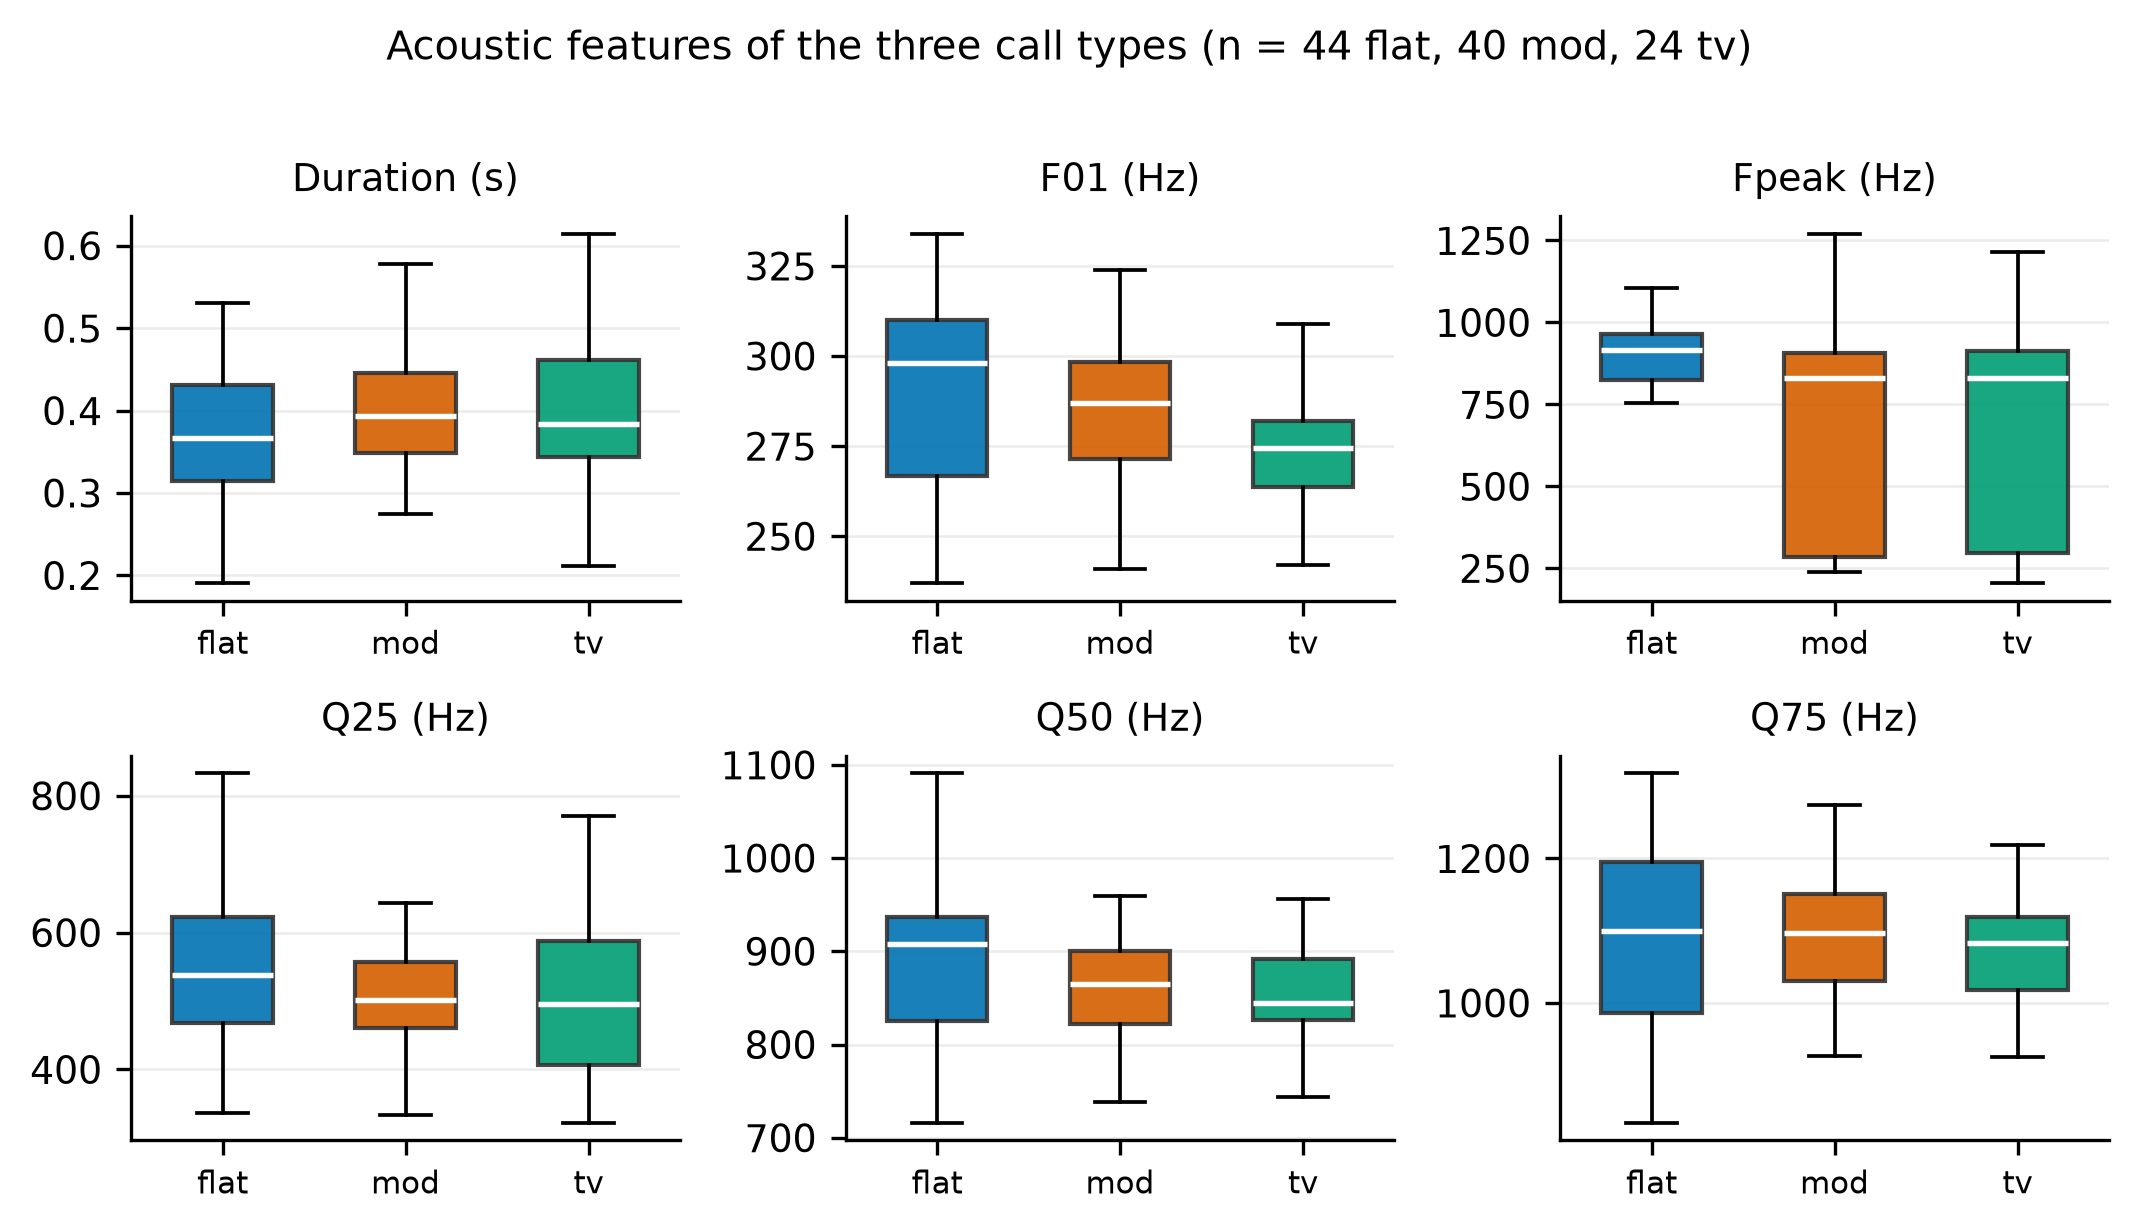
\includegraphics[width=0.78\textwidth]{figs/fig1_features.png}
  \caption{Distributions of the six shared acoustic features by call type. Boxes show the
  interquartile range, the white line the median, and whiskers extend to 1.5 times the
  interquartile range.}\label{fig:q1-features}
\end{figure}

Two features of the table deserve comment before any test is run. First, duration is almost
constant across types (medians 0.367, 0.394 and 0.383 s), so it cannot carry much discriminative
information. Second, the peak frequency has a strongly skewed distribution for modulated and
two-voice calls: the medians are 831 and 830 Hz, but the lower quartiles fall to about 290 Hz
and the means (667 and 676 Hz) sit far below the medians. A handful of low-frequency outliers
therefore inflates the variance, which is why the rank-based tests below are preferable to any
analysis of means.

\subsection{Two nonparametric tests}

We first apply a Kruskal--Wallis test to each of the six shared features and correct the six
$p$-values with the Holm procedure. Only the features that survive this omnibus correction are
then examined pairwise with Mann--Whitney $U$ tests, which are themselves Holm-corrected together
with the modulated--two-voice comparison of pulse rate. Table~\ref{tab:q1-kw} gives the omnibus
results.

\begin{table}[htbp]
  \centering
  \caption{Kruskal--Wallis tests across the three call types, Holm-corrected over six features.}\label{tab:q1-kw}
  \small
  \begin{tabular}{lrrr}
    \toprule
    Feature & $H$ (2 df) & Holm-adjusted $p$ & $\varepsilon^2$ \\
    \midrule
    Duration & 2.523 & 0.850 & 0.005 \\
    $F_{01}$ & 9.144 & 0.052 & 0.068 \\
    Fpeak & 12.280 & 0.013 & 0.098 \\
    Q25 & 2.157 & 0.850 & 0.001 \\
    Q50 & 6.425 & 0.161 & 0.042 \\
    Q75 & 0.520 & 0.850 & 0.000 \\
    \bottomrule
  \end{tabular}
\end{table}

Only peak frequency survives correction. The first fundamental is marginal ($p=0.052$) and the
median frequency does not survive ($p=0.161$), even though both show a monotone decrease from
flat to modulated to two-voice. The effect sizes tell the same story: $\varepsilon^2=0.098$ for
peak frequency against 0.068 for $F_{01}$ and 0.042 for Q50, and essentially zero for duration,
Q25 and Q75.

\begin{table}[htbp]
  \centering
  \caption{Pairwise Mann--Whitney tests for the features examined, Holm-corrected. Rank-biserial
  $r$ is positive when the first type tends to take larger values.}\label{tab:q1-pair}
  \small
  \begin{tabular}{llrr}
    \toprule
    Feature & Comparison & Adjusted $p$ & Rank-biserial $r$ \\
    \midrule
    Fpeak & flat vs mod & 0.0051 & 0.409 \\
    Fpeak & flat vs tv & 0.0314 & 0.379 \\
    Fpeak & mod vs tv & 0.956 & $-0.009$ \\
    PulseRate & mod vs tv & 0.557 & $-0.179$ \\
    \bottomrule
  \end{tabular}
\end{table}

The pairwise tests confirm where the separation lies, and the pattern is not the one a casual
reading of the medians would suggest. Flat
calls differ from both modulated and two-voice calls in peak frequency, but modulated and
two-voice calls do not differ from each other. The difference between call types is therefore
carried mainly by the position of the spectral peak, and only secondarily by $F_{01}$; once flat
is separated, the remaining two types are acoustically close on all continuous descriptors.

\subsection{Classification and the leakage trap}

The problem asks for a classifier and for the macro-averaged $F_1$, not accuracy alone, because
the classes are unbalanced (44/40/24 against a majority-class baseline of 0.407). We fit a random
forest and a multinomial logistic regression under two feature scopes. The \emph{shared} scope
uses the six features available for all calls; the \emph{full} scope adds the presence indicators
for $F_{02}$ and for the pulse rate, together with their missing-value flags. Both are evaluated
with stratified five-fold cross-validation repeated five times, with hyper-parameters tuned by an
inner three-fold split, and additionally by holding out whole recording dates.

\begin{table}[htbp]
  \centering
  \caption{Classification performance (mean over five repeats of stratified five-fold
  cross-validation).}\label{tab:q1-cv}
  \small
  \begin{tabular}{llrrrrr}
    \toprule
    Scope & Model & Accuracy & Macro-$F_1$ & Recall flat & Recall mod & Recall tv \\
    \midrule
    Shared & Random forest & 0.470 & 0.458 & 0.523 & 0.450 & 0.408 \\
    Shared & Logistic & 0.385 & 0.373 & 0.482 & 0.265 & 0.408 \\
    Full & Random forest & 0.944 & 0.952 & 1.000 & 0.850 & 1.000 \\
    Full & Logistic & 0.939 & 0.947 & 0.986 & 0.850 & 1.000 \\
    \midrule
    \multicolumn{2}{l}{Date holdout, shared forest} & 0.389 & 0.363 & --- & --- & --- \\
    \multicolumn{2}{l}{Date holdout, full forest} & 0.944 & 0.952 & --- & --- & --- \\
    \bottomrule
  \end{tabular}
\end{table}

The gap between the two scopes is the most important result in this section, and it is a warning
rather than a success. The full-scope classifier reaches a macro-$F_1$ of 0.952 because the
presence of a second fundamental identifies two-voice calls perfectly and the presence of a pulse
rate identifies flat calls. That is label leakage: the ``feature'' is a restatement of the class.
The honest measure of acoustic separability is the shared-scope result, 0.458, which is only
slightly above the majority-class baseline and collapses to 0.363 when whole dates are held out.
We report both, and we do not claim that the call types are acoustically separable on continuous
descriptors alone.

Permutation importance and significance disagree in one place. Importance concentrates on
$F_{01}$ (0.084) and Q50 (0.033), with Fpeak lower (0.019); significance after Holm correction
selects Fpeak alone. The source analysis resolves this by combining the two views and reports
$F_{01}$, Q50 and Fpeak as the key shared indicators, which is the set carried into
Problems~2 and 3. The disagreement is interpretable rather than troubling: importance measures
how much a tree ensemble uses a feature given the others, whereas the rank test measures marginal
separation, and Fpeak separates flat from the other two while being largely redundant with
$F_{01}$ and Q50 once those are available.

\subsection{Information function and transmission robustness}

The three call types are not three labels for the same signal. The acoustic evidence suggests a
division of labour that the later sections test behaviourally.

Flat calls have the highest first fundamental (298 Hz) and the highest peak frequency (916 Hz),
the narrowest spectral spread, and no pulse structure. A pure tone of this kind is easy to
localise and easy to detect against low-frequency noise, but it carries little fine structure, so
it can signal presence more easily than identity.

Modulated calls add a pulse rate (median 28.4 Hz) and a broader peak distribution. The temporal
modulation provides redundancy in the time domain, which is what survives when the spectrum is
distorted by multipath propagation.

Two-voice calls carry a second fundamental at 303.5 Hz in addition to the first at 274.5 Hz. This
is the only structural feature that is unique to a call type, and it is the feature that makes
the full-scope classifier look excellent. Its function is plausibly redundancy across frequency
bands: if one band is masked by noise, the other still carries the pattern.

These interpretations are hypotheses, not results, and we label them as such. What the data
establish is narrower: the three types differ in where their spectral energy sits and in whether
they carry a second band or a pulse train. Whether those differences matter for transmission is
the question of Section~\ref{sec:q2}, and whether they matter for behaviour is the question of
Section~\ref{sec:q3}.

\paragraph{Hand-off to later sections.}
Three indicators are carried forward: $F_{01}$ as the carrier of the fundamental, Fpeak as the
most statistically distinct descriptor, and Q50 as a robust summary of spectral placement. The
structural indicators ($F_{02}$ present, pulse rate present) are carried forward as \emph{call
type definitions}, not as acoustic covariates, precisely because they would leak the label.
